\documentclass{article}
\usepackage{graphicx} % Required for inserting images
\usepackage{amsmath}
\usepackage{amsfonts}

\title{ICPC Template Math}
\author{Hoa Le}
\date{October 2024}

\begin{document}

% Written by Anders Sjoqvist and Ulf Lundstrom, 2009
% The main sources are: tinyKACTL, Beta and Wikipedia

\chapter{Mathematics}

\section{Trigonometry}
\begin{align*}
\sin(v+w)&{}=\sin v\cos w+\cos v\sin w\\
\cos(v+w)&{}=\cos v\cos w-\sin v\sin w\\
\end{align*}
\begin{align*}
\tan(v+w)&{}=\dfrac{\tan v+\tan w}{1-\tan v\tan w}\\
\sin v+\sin w&{}=2\sin\dfrac{v+w}{2}\cos\dfrac{v-w}{2}\\
\cos v+\cos w&{}=2\cos\dfrac{v+w}{2}\cos\dfrac{v-w}{2}
\end{align*}
\[ (V+W)\tan(v-w)/2{}=(V-W)\tan(v+w)/2 \]
where $V, W$ are lengths of sides opposite angles $v, w$.
\begin{align*}
	a\cos x+b\sin x&=r\cos(x-\phi)\\
	a\sin x+b\cos x&=r\sin(x+\phi)
\end{align*}
where $r=\sqrt{a^2+b^2}, \phi=\operatorname{atan2}(b,a)$.

\section{Geometry}

\subsection{Triangles}
Side lengths: $a,b,c$\\
Semiperimeter: $p=\dfrac{a+b+c}{2}$\\
Area: $A=\sqrt{p(p-a)(p-b)(p-c)}$\\
Circumradius: $R=\dfrac{abc}{4A}$\\
Inradius: $r=\dfrac{A}{p}$\\
Length of median (divides triangle into two equal-area triangles): $m_a=\tfrac{1}{2}\sqrt{2b^2+2c^2-a^2}$\\
Length of bisector (divides angles in two): $s_a=\sqrt{bc\left[1-\left(\dfrac{a}{b+c}\right)^2\right]}$\\
Law of sines: $\dfrac{\sin\alpha}{a}=\dfrac{\sin\beta}{b}=\dfrac{\sin\gamma}{c}=\dfrac{1}{2R}$\\
Law of cosines: $a^2=b^2+c^2-2bc\cos\alpha$\\
Law of tangents: $\dfrac{a+b}{a-b}=\dfrac{\tan\dfrac{\alpha+\beta}{2}}{\tan\dfrac{\alpha-\beta}{2}}$\\

\subsection{Quadrilaterals}
With side lengths $a,b,c,d$, diagonals $e, f$, diagonals angle $\theta$, area $A$ and
magic flux $F=b^2+d^2-a^2-c^2$:

\[ 4A = 2ef \cdot \sin\theta = F\tan\theta = \sqrt{4e^2f^2-F^2} \]

 For cyclic quadrilaterals the sum of opposite angles is $180^\circ$,
$ef = ac + bd$, and $A = \sqrt{(p-a)(p-b)(p-c)(p-d)}$.

\subsection{Spherical coordinates}
\begin{center}
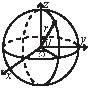
\includegraphics[width=25mm]{content/math/sphericalCoordinates}
\end{center}
\[\begin{array}{cc}
x = r\sin\theta\cos\phi & r = \sqrt{x^2+y^2+z^2}\\
y = r\sin\theta\sin\phi & \theta = \textrm{acos}(z/\sqrt{x^2+y^2+z^2})\\
z = r\cos\theta & \phi = \textrm{atan2}(y,x)
\end{array}\]

\section{Sums}
\[ c^a + c^{a+1} + \dots + c^{b} = \frac{c^{b+1} - c^a}{c-1}, c \neq 1 \]
\begin{align*}
	1^3 + 2^3 + 3^3 + \dots + n^3 &= \frac{n^2(n+1)^2}{4} \\
	1^4 + 2^4 + 3^4 + \dots + n^4 &= \frac{n(n+1)(2n+1)(3n^2 + 3n - 1)}{30} \\
\end{align*}

\section{Combinatorics}

\subsection{Catalan numbers}
\begin{itemize}
    \item Number of correct bracket sequence of length 2n.
    \item Number of stack-sortable permutation of length n.
    \item Number of ways to cut a polygon with n + 2 sides into n triangles with no cut crossing each other.
    \item Number of permutation with no three-term increasing subsequence (no i such that $a_i < a_{i + 1} < a_{i + 2}$).
    \item Number of full binary trees with n + 1 leaves.
    \item $1, 1, 2, 5, 14, 42, 132, 429, 1430, 4862, 16796, 58786, ...$
\end{itemize}
\begin{align*}
    C_n = \binom{2n}{n} - \binom{2n}{n+1} = \frac{1}{n+1} \binom{2n}{n} = \frac{1}{2n+1} \binom{2n+1}{n}
\end{align*}

\subsection{Motzkin numbers}
\begin{itemize}
    \item Number of different ways of drawing non-intersecting chords between n points on a circle.
    \item Number of \textbf{positive} integer sequences of length n + 1 in which the opening and ending elements are 1, and the difference between any two consecutive elements is -1, 0 or 1.
    \item Number of \textbf{positive} integer sequences of length n - 1 in which the opening and ending elements are either 1 or 2, and the difference between any two consecutive elements is -1, 0 or 1.
    \item $1, 1, 2, 4, 9, 21, 51, 127, 323, 835, ...$
\end{itemize}
\begin{align*}
    M_n = M_{n-1} + \sum_{i=0}^{n-2} M_i M_{n-2-i} = \frac{2n+1}{n+2} M_{n-1} + \frac{3n-3}{n+2} M_{n-2}
\end{align*}

\subsection{Schröder numbers}
\begin{itemize}
    \item Number of ways to connect n points on a circle with non-crossing edges, where edges can either be straight or touch
    \item Number of ways to move from (0,0) to (n,n) with 3 kinds of steps: (1,0), (1,1), (0,1) and never goes above the SW-NE diagonal.
    \item Number of ways to move from (0, 0) to (2n, 0) with 3 kinds of steps: (1,0), (1,1), (0,1) and never goes below the x-axis.
    \item Number of ways to divide a rectangle into n + 1 smaller rectangles using n cuts through n points given inside the rectangle in general position, each cut intersecting one of the points and dividing only a single rectangle in two.
    \item $1, 2, 6, 22, 90, 394, 1806, 8558, ...$
\end{itemize}
\begin{align*}
    S_n = \frac{6n - 3}{n + 1} S_{n-1} - \frac{n - 2}{n + 1} S_{n-2}
\end{align*}

\subsection{Bell numbers}
\begin{itemize}
\item Number of partitions of a set of n items into non-empty disjoint subsets.
\item $1, 1, 2, 5, 15, 52, 203, 877, 4140, ...$
\end{itemize}
\begin{align*}
    B_{n+1} = \sum_{k=0}^{n} \binom{n}{k} B_k\\
    B_{p+n} \equiv B_n + B_{n+1} \pmod{p}\\
    B_{p^m+n} \equiv mB_n + B_{n+1} \pmod{p}
\end{align*}

\subsection{Ordered Bell numbers --- Fubini numbers}
\begin{itemize}
\item Number of ways to arrange elements into a sequence allowing ties, such as might arise as the outcome of a horse race.
\item Number of ordered multiplicative partition of a positive integer, or its representation of the number as a product of one or more of its divisors.
\item $1, 1, 3, 13, 75, 541, 4683, ...$
\end{itemize}
\begin{align*}
    a(n) = \sum_{i=1}^{n} \binom{n}{i} a(n-i)\\
    a(n-1) a(n+1) \geq a(n)^2
\end{align*}

\subsection{Lah numbers}
\begin{itemize}
    \item Number of ways a set of n elements can be partitioned into k non-empty linearly ordered subsets.
    \item $L(0, 0) = 1$
    \item $L(1, k) = 0, 1$
    \item $L(4, k) = 0, 24, 36, 12, 1$
\end{itemize}
\begin{align*}
    L(n, k) = \binom{n-1}{k-1} \frac{n!}{k!}
\end{align*}

\subsection{Delannoy numbers}
\begin{itemize}
    \item Number of ways to move from (0,0) to (m,n) with 3 kinds of steps: (1,0), (1,1), (0,1)
    \item $D(0, k) = 1, 1, 1, 1, ...$
    \item $D(3, k) = 1, 7, 25, 63, ...$
\end{itemize}
\begin{align*}
    D(m,n) = \sum_{k=0}^{\min(m,n)} \binom{m+n-k}{m} \binom{m}{k} = \sum_{k=0}^{\min(m,n)} \binom{m}{k} \binom{n}{k} 2^k
\end{align*}

\subsection{Eulerian numbers}
\begin{itemize}
    \item Number of permutations of the numbers 1 to n in which exactly k elements are greater than the previous element (permutations with k position i where $a_i < a_{i + 1}$)
    \item $A(0, 0) = 1$
    \item $A(5, k) = 1, 26, 66, 26, 1$
\end{itemize}
\begin{align*}
    A(n,k) = (n - k)A(n-1, k-1) + (k+1)A(n-1, k) = \sum_{i=0}^{k} (-1)^i \binom{n+1}{i}(k+1-i)^n
\end{align*}

\subsection{Narayana numbers}
\begin{itemize}
    \item Number of ways to move from (0, 0) to (2n, 0) with 2 kinds of steps: (1, 1), (1, -1) and never goes below the x-axis, with exactly k peaks.
    \item $A(1, 1) = 1$
    \item $A(5, k) = 1, 10, 20, 10, 1$
\end{itemize}
\begin{align*}
    N(n,k) = \frac{1}{n} \binom{n}{k} \binom{n}{k-1}
\end{align*}

\subsection{Stirling numbers of the first kind}
\begin{itemize}
    \item Number of permutation of size n with k permutation cycles.
    \item $s(0, 0) = 1$
    \item $s(5, k) = 0, 24, 50, 35, 10, 1$
\end{itemize}
\begin{align*}
    \left[ {n+1 \atop k} \right] = n \left[ {n \atop k} \right] + \left[ {n \atop k-1} \right]
\end{align*}

\subsection{Stirling numbers of the second kind}
\begin{itemize}
    \item Number of ways to partition a set of n objects into k non-empty subsets.
    \item $S(0, 0) = 1$
    \item $S(5, k) = 0, 1, 15, 25, 10, 1$
\end{itemize}
\begin{align*}
\left\{ {n+1 \atop k} \right\} = k \left\{ {n \atop k} \right\} + \left\{ {n \atop k-1} \right\} \\
\left\{ {n \atop k} \right\} = \frac{1}{k!} \sum_{i=0}^{k} (-1)^{k-i} \binom{k}{i} i^n
\end{align*}

\end{document}
